\cotefile{36}
\scanpage{10}
\handwritten{\unsure{I|1}) \uline{Le théorème de Griffiths par voie algébrique.}}

1.\quad Soit
\[
f:Y\handwritten{\longrightarrow}S
\]
un morphisme propre et lisse de schémas, avec $S$ \inserted{\handwritten{régulier,}} connexe à caractéristiques résiduelles toutes $\handwritten{\ne\ell}$ (nombre premier fixé). Soit $s\handwritten{\in}S$, $\bar s$ un point géométrique au dessus de $s$. Soi\deleted{\unsure{t}}\handwritten{t} $F$ un faisceau $\handwritten{\ell}$-adique constant tordu sur $S$ (en pratique, un faisceau de la forme $\underline{Z}_{\handwritten{\ell}}(i)$ ), et $x$ une classe de cohomologie
\[
x\handwritten{\in}H^{\deleted{N}\handwritten{\unsure{m}}}(Y,\deleted{\unsure{f^*(F)|f^*F}}\handwritten{F_Y})\ .
\]
Disons que $x$ est \uline{primitive} si son image dans $H^0(S,R^m f_{\handwritten{*}}\handwritten{(\unsure{F|f})})\deleted{\unsure{(F)|F)}}$ est nulle, ou ce qui revient au même par le th. de spécialisation de la cohomologie, si son image dans $H^{\deleted{N}\handwritten{m}}(Y_{\bar s},F_{\bar s})$ est nulle. Alors la suite spectrale de Leray pour $f$ nous donne un élément
\[
u(x)\handwritten{\in}{\unsure{\mathbb{E}|E}}_2^{1,\deleted{\unsure{N-1|m-1}}\handwritten{m-1}}=H^1(S,R^{\deleted{\unsure{m|N}}\handwritten{m-1}}_{\deleted{\unsure{2}}}f_{\deleted{\unsure{f}}\handwritten{*}}(F_{\handwritten{Y}}))\ .
\]
Donnons une propriété fonctorielle générale de cette classe $u(x)$. Pour ceci, soit $Y'$ lisse et propre sur $S$, et
\[
\unsure{\mathbb{Z}|Z|z}\handwritten{\in}H^N(Y\mathbin{\mathrm{x}}_S Y',G),
\]
de sorte que par le formalisme des correspondances cohomologiques, $z$ définit une application
\[
x'\handwritten{\longmapsto}Z(x'): \quad H^{m'}(Y',F')\handwritten{\longrightarrow}H^m(Y,F),
\]
si on suppose $m=m'+N-\deleted{\unsure{\dim(Y'/S)|\dim(X'/S)}}\handwritten{2d'}$, et qu'on a un accouplement $F'\handwritten{\otimes}G\handwritten{\longrightarrow}F(d')$ (NB $d'$ est la dimension relative de $Y'$ sur $S$, supposée constante, et $(d')$ désigne le twist de Tate\deleted{\unsure{xx|de}}; $F'$ et $G$ désignent des faisceaux $\handwritten{\ell}$-adiques constants tordus \inserted{\handwritten{sur $S$}} tout comme $F$). Ceci dit, si $x'$ est primitive, alors il en est évidemment de même de $x=Z(x')$, et on aura de plus
\[
u(Z(x'))=Z(u(x'))\ ,
\]
où le deuxième membre s'explicite en notant que $Z$ définit également, par
% archive sheet number: 9
\scanpage{11}
\handwritten{\mspage{2}}
localisation étale sur $S$, un homomorphisme
\[
a'\handwritten{\longmapsto}Z(a'):\quad R^{m'-1}f'_{\handwritten{*}}({\unsure{\mathbb{E}|\mathbb{F}|E|F|C|G}}_{Y'})\handwritten{\longrightarrow}R^{m-1}f_{\handwritten{*}}(F_Y)\ ,
\]
et par suite un homomorphisme (encore noté par $Z$) des $H^1(S,\ )$ pour les drux membres.

Nous allons appliquer ceci au cas où $Y'$ est une courbe relative $C$ sur $S$, $m'=2$, $x'$ est la classe de cohomologie
\[
x'\handwritten{\in}H^{\handwritten{2}}(C,\underline{Z}_{\handwritten{\ell}}(1))
\]
défini par un diviseur relatif de la forme $t_1(S)-t_0(S)$, où $t_1$ et $t_0$ sont deux sections de $C$ sur $S$. Supposant $C$ à fibres géométriques connexes on voit donc que $x'$ est primitif. (NB on pourrait prendre aussi bien n'importe quel diviseur relatif de degré relatif nul.) On prendra pour $Z$ la classe de cohomologie
\[
Z\handwritten{\in}H^{2n}(Y\mathbin{\mathrm{x}}_S C,\underline{Z}_{\handwritten{\ell}}(n))
\]
associée à un cycle algébrique sur $Y\mathbin{\mathrm{x}}_S C$ de codimension $n$, qu'on notera aussi $Z$. (NB pour que cette classe de cohomologie soit vraiment définie en l'état actuel de la Science, il faut faire des hypothèses restrictives genre $S$ de type fini sur un corps, ou $S$ excellent de caractéristique \unsure{nulle} ou le dycle $Z$ un cycle ``relatif'' i.e. de codimension $\handwritten{\leq}n$ fibre par fibre

Sous ces conditions, $x$ est la classe de cohomologie
\[
x\handwritten{\in}H^{2n}(Y,\underline{Z}_{\handwritten{\ell}}(n))
\]
associée au cycle algébrique
\[
z=Z(t_1)-Z(t_0)
\]
sur $Y$. (NB on suppose que les intersections écrites ont un sens, ou qu'on travaille avec des \uline{classes} de cycles de façon qu'elles en aient un, - ce dernier cas supposant (toujours en l'état actuel de la Science) \unsure{què|qué|que}\deleted{\unsure{ax|xx}} $S$ est de type fini sur un corps.
% archive sheet number: 10
\scanpage{12}
\handwritten{\mspage{3}}
Ceci posé, le cycle $Z$ (ou plutôt, sa classe de cohomologie) définit un homomorphisme naturel
\[
Z:\quad R^1g_{\handwritten{*}}(\underline{Z}_{\handwritten{\ell}}(1))\handwritten{\longrightarrow}R^{\unsure{2|a}n-1}f_{\handwritten{*}}(\underline{Z}_{\handwritten{\ell}}(n))\ ,\tag*{(*)}
\]
d'où un homomorphisme
\[
Z:\quad H^1(S,R^1g_{\handwritten{*}}(\underline{Z}_{\handwritten{\ell}}(1)))\handwritten{\longrightarrow}H^1(S,R^{2n-1}f_{\handwritten{*}}(\underline{Z}_{\handwritten{\ell}}(n)))\ ,\tag*{(**)}
\]
et la compatibilité générale énoncée plus haut nous dit que $u(x)=u(c\handwritten{l}(z))$ n'est autre que l'image de $u(x')$ du premier membre de \deleted{\unsure{(*)x|(*)}} (**). Nous \unsure{aurons|avrons} besoin simplement pour la suite de savoir que \uline{si l'homo\deleted{\unsure{morphismo|morphisme}}morphisme\deleted{\unsure{xx}}} (*) \uline{est nul} (\uline{ou ce qui revient au même, si l'homomorphisme correspondant sur les fibres géométriques en} $\bar s$ \deleted{est}
\[
H^1(C_{\bar s},\underline{Z}_{\handwritten{\ell}}(1))\handwritten{\longrightarrow}H^{2n-1}(Y_{\bar s},\underline{Z}_{\handwritten{\ell}}(n))\tag*{(* bis)}
\]
\uline{est nulle}), \uline{alors il en est de même de} $u(x)\handwritten{\in}H^1(S,R^{2n-1}f_{\handwritten{*}}(\underline{Z}_{\handwritten{\ell}}(n)))$.

2.\quad Soit
\[
i:Y\handwritten{\longrightarrow}X
\]
un morphisme de schémas \deleted{projectifs}\handwritten{\unsure{propres}} et lisses sur un corps algébriquement clos $k$, $n$ un entier. On \deleted{suppose} considère l'homomorphisme
\[
i^{\handwritten{*}}:\quad H^{2n-1}(X,\underline{\deleted{Z}\handwritten{Q}}_{\handwritten{\ell}}(n))\handwritten{\longrightarrow}H^{2n-1}(Y,\underline{\deleted{Z}\handwritten{Q}}_{\handwritten{\ell}}(n))\ ,\tag*{\handwritten{(***)}}
\]
et on suppose:

a)\quad Il existe un homomorphisme en sens inverse $\unsure{v^*|v*}$, dont la restriction à l'image de\deleted{\unsure{xxx|xx}} $i^*$ soit un inverse à droite de $i^*$, et qui soit ``algébrique'' i.e. donné par un cycle algébrique sur $Y\mathbin{\mathrm{x}}X$. (NB Cette hypothèse est un cas particulier des ``conjectures standart'', donc est sans doute touhours vérifiée; elle est vérifiée en tous cas si $i$ est l'i\deleted{\unsure{x}}nclusion d'une section hyperplane dans $X$, lorsque l'opération $\handwritten{\Lambda}$ sur \deleted{\unsure{X est|Xxest}} la cohomologie de $X$ est algébrique, \deleted{\unsure{ce|xx}} \inserted{propriété} qu'on sait vérifier dans de très nombreux cas, par exemple lorsque $X$ se remonte en car. zéro avec sa polarisation.)
% archive sheet number: 11
\scanpage{13}
\handwritten{\mspage{4}}
b)\quad Pour toute courbe algébrique (propre, lisse, connexe) $\unsure{\mathbb{C}|C}$ sur $k$, et tout cycle algébrique $Z$ sur $Y\mathbin{\mathrm{x}}C$ de codimension $n$, l'homomorphisme correspondant
\[
Z:H^1(C)\underline{\deleted{Z}\handwritten{Q}}_{\handwritten{\ell}}(1))\handwritten{\longrightarrow}H^{2n-1}(Y,\underline{Q}_{\handwritten{\ell}}(n))
\]
a son image dans celle de $i^{\handwritten{*}}$ de (***). (NB Si on admet le yoga des motifs, justifiable par les``conjectures standard'', \unsure{cetté|cette}\deleted{\unsure{même|xxxxé}} condition signifie que le \inserted{\handwritten{plus grand}} morceau \deleted{\unsure{du|de|dx}} ``de niveau 1'' du motif \deleted{Coker} ayant comme réalisation $\handwritten{\ell}$-adique $\mathrm{Coker}\ i^{\handwritten{*}}$ est nul).

\uline{Sous ces conditions}, \uline{pour tout cycle algébrique} $z\handwritten{\in}Z^n(Y)$ \uline{qui est algébriquement équivalent à zéro}, \uline{il existe un cycle} $z'\handwritten{\in}Z^n(X)$ \uline{algébriquement équivalent à zéro}, et \uline{un} $z''\handwritten{\in}Z^n(Y)$, tels que
\[
z=i^{\handwritten{*}}(z')+z''\tag*{a')}
\]
b')\quad \deleted{\unsure{l'hom|l'homx|Xhomx}} $z''=Z^{\handwritten{''}}(t_1)-Z^{\handwritten{''}}(t_0)$, où $Z''$ est un \inserted{$\underline{Q}$-}cycle \uline{de codimension} $n$ \uline{sur un}\deleted{\unsure{e courbe|courbe}} \uline{produit} $\deleted{\unsure{C|Cx}}\deleted{X}\handwritten{Y}\mathbin{\mathrm{x}}C$, \uline{induisant un homomorphisme} \uuline{nul} \deleted{\unsure{de|dx}} $H^1(C,\underline{Q}_{\handwritten{\ell}}(1))\handwritten{\longrightarrow}H^{2n-1}(Y,\underline{Q}_{\handwritten{\ell}}(n))$.

Démonstration immédiate : on écrit $z=Z(t_1)-Z(t_0)$ avec $Z\handwritten{\in}Z^n(Y\mathbin{\mathrm{x}}C)$, ce $Z$ définit un homomorphisme $Z:H^1(C)\handwritten{\longrightarrow}H^{2n-1}(Y)$, \deleted{dont le} qui par hypothèse b) tombe dans $\mathrm{Im}\ i^{\handwritten{*}}$ donc par \unsure{hypthèse|hypothèse} a) est égal au composé $(iv)Z=i(vZ)$, or $vZ:H^1(C)\handwritten{\longrightarrow}H^{2n-1}(X)$ est algébrique puisque $v$ l'est, donc donné par un cycle algébrique $Z'$ sur $X\mathbin{\mathrm{x}}C$, et si on pose $Z''=Z-(i\mathbin{\mathrm{x}}\mathrm{id}_C)^{\handwritten{*}}(Z\handwritten{'} )$, on aura par construction que $Z''$ induit l'homomorphisme nul $H^1(C)\handwritten{\longrightarrow}H^{2n-1}(Y)$. \deleted{D'autre part} Il suffit alors de poser $\unsure{z'|\mathbb{Z}'|Z'}=Z'(t_1)-Z'(t_0)$, $z''=Z''(t_1)-Z''(t_0)$.

3.\quad Mettant ensemble les réflexions de 1) et 2), on trouve ceci. On se donne des schémas propres et lisses $X$ et $Y$ sur $S$ \inserted{\handwritten{régulier,}} connexe, et un $S$-morphisme
\[
i:Y\handwritten{\longrightarrow}X\ .
\]
% archive sheet number: 12
\scanpage{14}
\handwritten{\mspage{5}}
Onnsuppose \inserted{a) et b) vérifiés pour le morphisme $i_{\bar s}:X_{\bar s}\handwritten{\longrightarrow}X_{\bar s}$ induit} \deleted{que le morphisme induit} pour lesfibres en $\bar s$ (point géométrique \deleted{fixé} de $S$\deleted{, qu'on a intérêt à prendre} au dessus da point \uline{générique} de $S$) \deleted{si $S$ est irréductible pour avoir le maximum de chances de \unsure{pouvoir que|pourvoir que} l'hypothèse sérieuse b). Soit $z$ un cycle a} \inserted{Soit} $z\handwritten{\in}Z^n(Y)$ tel que le cycle induit sur $Y_{\bar s}$ soit algébriquement équivalent à zéro, et à fortiori cohomologiquement équivalent à zéro. Donc da classe
\[
u(z)\handwritten{\in}H^1(S,R^{2n-1}f_{\handwritten{*}}(\underline{Z}_{\handwritten{\ell}}(n))
\]
est définie. Ceci posé, je dis que \uline{cette classe est \deleted{une classe de torsion} contenue dans} $i^{\handwritten{*}}(H^{\deleted{\unsure{0}}1}(S,R^{2n-1}\deleted{\unsure{f|g}}\handwritten{g}_{\handwritten{*}}({\unsure{\underline{Z}|\underline{Q}}}_{\handwritten{\ell}}(n)))$ \uline{modulo une classe de torsion}, du moins si on \deleted{suppose $S$ japonais de dimension 1, ou même} \deleted{\inserted{On applique 2) à $\unsure{i_{\bar s}|i}$}} \deleted{\inserted{si,}} se permet de remplacer $S$ par un ouvert non vide(restriction \deleted{sans doute}\inserted{probablement} inutile, mais cet énoncé nous suffira pour ce qu'on veut en faire).

Pour le voir, on applique 2) au morphisme $i_{\bar s}$. La courbe $C$ et le cycle $Z''$ peuvent de définit déjà sur une extension finie $K$ de $k(s)$, Un argument de trace permet de supposer que $K=k(s)$, et \deleted{quitte à prendre l'adhérence du cycle} on peut supposer que $\unsure{\mathbb{C}|C|Z}$ \deleted{et $Z$} est une courbe propre et lisse relative sur $S$ lui-même, et $Z''$ un cycle sur $\unsure{\mathbb{X}|X|Y}\mathbin{\mathrm{x}}_S C$, \deleted{Alors} et que la formule $z=i^{\handwritten{*}}(z')+z''$ est valable sur $\unsure{\mathbb{X}|X|Y}\mathbin{\mathrm{x}}_S C$. Elle implique une décomposition analogue de $u(z)$, qui est la somme de $i^{\handwritten{*}}(u(z'))$ et de $u(z'')$, de sorte qu'il suffit de prouver que $u(z'')$ est nul. Or $u(z'')$ induit par \deleted{\unsure{d}}construction 2) l'homomorphisme nul $H^1(C_{\bar s})\handwritten{\longrightarrow}H^{2n-1}(Y_{\bar s})$. Im résulte donc bien de 1) que $u(z'')$ est nul, cqfd.

4.\quad Soient $X$ un schéma projectif et lisse de dimension $m$\inserted{\handwritten{sur $k$ Alg. clos}}, prenons un pinceau de Lefschetz, de façon à obtenir une variété éclatée non moins projective et lisse $\overset{\handwritten{\sim}}{X}$ et un morphisme
\[
\overset{\handwritten{\sim}}{f}:\overset{\handwritten{\sim}}{X}\handwritten{\longrightarrow}\deleted{\unsure{S|Sx}}P^1_k
\]
dont les fibres sont les sections hyp\deleted{\unsure{k|x}}erplanes du pinceau. Soit $\unsure{\mathbb{S}|S|U}$ un ouvert non vide de $P^1_k$ au dessus duquel $\overset{\handwritten{\sim}}{X}$ soit lisse, et soit $\handwritten{\unsure{j|f}}:Y=\overset{\handwritten{\sim}}{X}\handwritten{|}S\handwritten{\longrightarrow\unsure{S}}$.
% archive sheet number: 13
\scanpage{15}
\handwritten{\mspage{6}}
Soit $P^m(X)$ la partie primitive de la cohomologie $H^m(X,\underline{Q}_{\handwritten{\ell}})$, i.e. le noyau du composé
\[
H^m(X)\handwritten{\longrightarrow}H^m(\overset{\handwritten{\sim}}{X})\handwritten{\longrightarrow}H^m(Y)\handwritten{\longrightarrow}H^0(S,R^m f_{\handwritten{*}}(\underline{Q}_{\handwritten{\ell}}))\ .
\]
On trouve donc grâce à I) un homomorphisme (dit ``de Griffiths'')
\[
P^m(X)\handwritten{\longrightarrow}H^1(S,R^{m-1}f_{\handwritten{*}}(\underline{Q}_{\handwritten{\ell}}))
\]
(en fait, on y pourrait remplacer $S$ par $P^1_k$, mais \deleted{\unsure{nous et|nous at}} peu importe ici)

D'ailleurs \deleted{\unsure{l'hom|lthom}} on a un homomorphisme d'immersion canonique
% Diagram objects and labels typed; all three arrows handwritten.
\diagram{\begin{tikzcd}[ampersand replacement=\&,column sep=small,row sep=small]
Y\handwritten{\arrow[rr]}\arrow[rr,phantom,"i"]\handwritten{\arrow[dr]}\arrow[dr,phantom,"f"']\&\&X_S\handwritten{\arrow[dl]}\arrow[dl,phantom,"g"]\\
\&S\&
\end{tikzcd}}\noindent ,
induisant
\[
i^{\handwritten{*}}:\quad H^1(S,R^{m-1}g_{\handwritten{*}}(\underline{Q}_{\handwritten{\ell}}))=H^1(S,H^{m-1}(X,\underline{Q}_{\handwritten{\ell}}))\handwritten{\longrightarrow}H^1(S,R^{m-1}f_{\handwritten{*}}(\underline{Q}_{\handwritten{\ell}})).
\]
Ceci dit, \uline{l'image inverse par l'homomorphisme de Griffiths plus haut de} $\mathrm{Im}\ i^*$ \uline{est réduite à zéro}.

Ceci se fait par des calculs explicites essentiellement triviaux, compte tenu de la structure cohomologique connue d'une variété éclatée.

5.\quad Mettant ensemble 3) et 4), on trouve ceci:

\deleted{Sous} Avec les notations de 4), \inserted{supposant $m=2n$,} soit $s$ le point générique de $P^1_k$, et \uline{supposons que l'immersion} $Y_{\bar s}\handwritten{\longrightarrow}X\handwritten{\otimes}_k k(\bar s)$ de \uline{la section hyperplane générique} \deleted{dans} \uline{satisfasse aux conditions} a) et b) de 2).\deleted{(\unsure{Alors pour On|Alors pour où} suppose de plus $m=2n$} \uline{Alors pour tout} $z\handwritten{\in}Z^n(X)$ \uline{dont la restriction à} $Y_{\bar s}$ \uline{est algébriquement équivalent à zéro}, $z$ \uline{est cohomologiquement équivalent à zéro} (mod torsion). \deleted{\unsure{En d'autre|En d'autr}} Par suite, le groupe quotient du groupe des cycles cohomologiquement équivalents à zéro \deleted{mod torsion} sur $Y_{\bar s}$, modulo ceux qui sont algébriquement équivalents à zéro (groupe qui mérite le nom de \uline{groupe de Griffiths} $\mathrm{Grif}\handwritten{(}Y_{\bar s})$ de $Y_{\bar s_{\deleted{\unsure{x|k}}}}$),\deleted{contient} \unsure{tensorisé} par $\underline{Q}$, contient comme sous-espace le sous-espace $P^{2n}_{\mathrm{alg}}(X)$ formé des \unsure{classes} de cohomologie primitives sur $X$ qui sont \uline{algébriques}, - vectoriel qui a
% archive sheet number: 14
\scanpage{16}
\handwritten{\mspage{7}}
\margin{\handwritten{\figure{\begin{tikzpicture}[x=1cm,y=1cm]\draw[line width=0.8pt] (0,0.20)--(0.025,0.10)--(0.03,0);\end{tikzpicture}}}}
une nette tendance à être $\handwritten{\ne}0$.

6.\quad \deleted{Conjecture II} \uline{Conjecture}: pour $X$\inserted{$\handwritten{\subset}P^r_k$} fixé\deleted{\unsure{x}}, comme dans 5), \inserted{avec $n\handwritten{\geq}2$,} il existe un entier $d_0$ tel que pour tout pinceau \inserted{de Lefschetz \handwritten{assez général}} de hypersurfaces de degré $d\handwritten{\geq}d_0$ dans $P^r$, donnant une section générique $Y_{\bar s}$ avec $X$, l'inclusion $Y_{\bar s}\handwritten{\hookrightarrow}X_{\bar s}$ satisfait à la condition b) de 2) (le fait que la condition a) doive être vérifiée en tous cas étant de toutes façons justiciable de la conjecture d'algébraicité de la\deleted{opération} correspondance cohomologique $\handwritten{\Lambda}$ sur $X$).
\margin{\handwritten{\figure{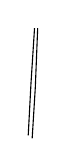
\begin{tikzpicture}[x=1cm,y=1cm]\draw (0.05,0)--(0.09,0.65)--(0.12,1.4);\draw (0,0.04)--(0.035,0.7)--(0.08,1.4);\end{tikzpicture}}}}

Nous allons examiner cette conjecture, en supposant déjà que le \deleted{\unsure{théorè|théoré}} théorème de Lefschetz ``vache'' soit vrai sur $X$, et que la correspondance $\handwritten{\Lambda}$ sur $X$ est algébrique. La théorie des cycles évanescents, qui sera prouvée dans SGA 7 cette année, donne alors ceci: L'orthogonal $E^{2n-1}\handwritten{\unsure{\deleted{(}|\ell}}$ de $H^{2n-1}(X)$, ponsidéré comme plongé dans $H^{2n-1}(Y_{\bar s})$, est un \uline{module simple sous l'action de} $\mathrm{Gal}(k(\bar s)/k(s))$, ainsi que \inserted{\handwritten{sous}} celle de tout sous-groupe \deleted{d'indice fini}\inserted{\handwritten{ouvert}}. (NB pour ce dernier fait, on utilise de façon essentielle qu'on est en dimension impaire $2n-1$, de sorte que les opérations de monodromie locale sont des transvections et non des symétries, \unsure{donc|dont} ne se tuent pas en passant à une puissance quelconque \ldots)Il s'ensuit déjà que \deleted{pour vérifier} la condition b)\deleted{il suffit de vérifier}\inserted{équivaut à dire} que $E^{2n-1}$ \uline{n'est pas tout entier de niveau} 1 . En caractéristique nulle, \deleted{il suffit} s'il était tout entier de niveau 1, \deleted{on en déduirait}\inserted{cela impliquerait} que les composantes de type $p,q$ de $E^{n-1}$ sont nulles sauf les deux composantes $(n,n-1)$ et $(n-1,n)$ (la réciproque étant vraie d'ailleurs si la conjecture de Hodge est vraie); cela \deleted{\unsure{implique que $H$|xxx implique que $H$}} signifie aussi que $\deleted{{\unsure{H|W}}^{\handwritten{2n-1}}(}$ $H^{p,q}(X)\handwritten{\hookrightarrow}H^{p,q}(Y)$ est un isomorphisme pour ces valeurs de $(p,q)$, en particulier que \deleted{il est} $H^{2n-1}(X,\underline{O}_X)\handwritten{\longrightarrow}H^{2n-1}(Y,\underline{O}_Y)$ est un isomorphisme\inserted{\handwritten{(car $n\geq2$)}}, ce qui n'est pas le cas pour $d$ grand (car la dimension du second membre tend vers $\handwritten{\infty}$ avec $d$). Cela prouve (par la méthode de Lefschetz, reprise par Griffiths) l'énoncé voulu en caractéristique nulle.
% archive sheet number: 15
\scanpage{17}
\handwritten{\mspage{8}}
\margin{\handwritten{\figure{\begin{tikzpicture}[x=1cm,y=1cm]\draw[gray,line width=0.4pt] (0,0.20)--(0,0.15);\draw[line width=1pt] (0.01,0.08)--(0.04,0.02);\end{tikzpicture}}}}
En caractéristique quelconque, on ne peut pour l'instant que donner des cas assez particuliers ou la conjecture soit vérifiée; par Katz, cela marche en tous cas pour \deleted{les}\inserted{\handwritten{$X$}} intersections complète\deleted{s}\inserted{\handwritten{et \deleted{\unsure{?}} un pinceau ``\unsure{en général|assez général}''}} (ce qui suffit pour faire marcher l'exemple minimal de Griffiths: $X$ quadrique dans $P^5$ ..). \deleted{La méthode} Pour vérifier que ${\unsure{\mathbb{E}|E}}^{2n-1}(Y_{\bar s})$ n'est pas de niveau 1, on constate aisément qu'il suffit de vérifier qu'il existe \uline{un} point $t$ du pinceau tel que $\mathbb{E}^{2n-1}(Y_{\bar t})$ ne soit pas de niveau 1 (il faut utiliser pour ceci le critère de Néron-Ogg-Chafarévitch de bonne réduction des VA; la triste vérité est que je ne sais pas \deleted{montrer}\inserted{montrer de façon générale}, même en \deleted{\unsure{termes|fermes}} admettant les conjectures standard, que le niveau d'un motif ne peut que diminuer par spécialisation \ldots) Quitte à écrire $k$ comme limite d'anneaux de type fini au sens absolu, la même observation est d'ailleurs valable, en se spécialisant sur un corps fini. Or dans ce cas, le niveau 1 implique\inserted{\handwritten{(et est \unsure{peut-être équivalent à})}} la divisibilité \inserted{\handwritten{par ${\unsure{1|q|p}}^{n-1}$}} des valeurs propres de frobenius opérant sur $\mathbb{E}^{2n-1}(Y_{\bar t})$ \deleted{par $q^{n-1}$} ($q=\mathrm{card}\ k(t)$), et il suffit donc de trouver $t$ tel que l'une des valeurs propres de frobenius soit une unité $p$-adique. C'est ce que Katz vérifie dans divers cas par une utilisation astucieuse de La formule de Lefschetz-Woodshole-Verdier.

7.\quad Le procédé de Katz. A lui de jouer ....
% archive sheet number: 16
\scanpage{18}
\handwritten{\mspage{9}}
\margin{\handwritten{\unsure{non}, pas tout à fait !}}
% The upper marginal note points to the encircled words « vais prouver ».
7. Je \parbox[c]{3.4cm}{\figure{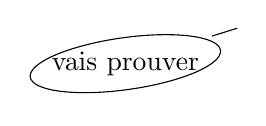
\begin{tikzpicture}[x=1cm,y=1cm]\node at (0,0) {vais prouver};\handwritten{\draw[rotate=8] (0,0) ellipse (1.22cm and 0.33cm);\draw (1.10,0.35)--(1.42,0.45);}\end{tikzpicture}}} la conjecture du n°6 pour des pinceaux de Lefschetz \deleted{\uline{Théorème}} assez généraux d'hypersurfaces de grand degré, en adaptant la méthode utilisée par Katz pour les intersections complètes. Nous allons prouver:

\margin{\handwritten{\unsure{pas prouvé} \unsure{sous cette} forme forte\figure{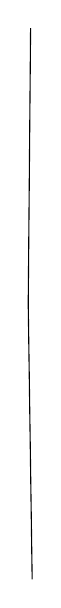
\begin{tikzpicture}[x=1cm,y=1cm]\draw (0.05,0)--(0,3.5)--(0.03,7);\end{tikzpicture}}}}
\uline{Théorème} 7.1. Soit $X\handwritten{\subset}P^r_k$ un schéma projectif équidimensionnel de Cohen-Macaulay, de dimension $n\handwritten{>}0$, sur un corps $k$ de car. $p\handwritten{>}0$. Il existe alors un entier $d_0\handwritten{>}0$ tel que, pour tout $d\handwritten{\geq}d_0$, si $Y$ est la section de $X$ par la\deleted{section} hypersurface générique de degré $d$, définie sur l'extension $k'=k(t_0,\ldots,t_r)$ de $k$, on ait la propriété qui suit\deleted{\unsure{e|x}}. On désigne par $E_0(Y)$ le conoyau de $H^{n-1}(X_{k'},\underline{O}_{X_{k'}})\handwritten{\longrightarrow}H^{n-1}(Y,\underline{O}_Y)$, qui est \deleted{muni d'un} un vectoriel de dimension finie sur $k'$, muni\deleted{\unsure{e|x}} de l'homomorphisme $p$-linéaire de frobenius $E_0(Y)^{(p)}\handwritten{\longrightarrow}E_0(Y)$ (prov\deleted{\unsure{i|x}}enant de la puissance p.ème sur les faisceaux de coefficients $\underline{O}_{X_{k'}}$, $\underline{O}_Y$). Soit \inserted{$V=$}$E_0(Y)_{ss}$ la partie semi-simple de $E_0(Y)$, i.e. le plus grand sous-espace \inserted{$V$} stable par frobenius et sur lequel frobenius induise un morphisme surjectif $V^{(p)}\handwritten{\longrightarrow}V$.

Considérons la représentation correspondante de $\unsure{G'|G}=\mathrm{Gal}(\bar k'/k')$ dans le vectoriel \inserted{$V_0$} de dim\deleted{\unsure{m}}ension $s=\dim_{k'}V$ sur $\underline{F}_p$ formé\deleted{\unsure{e|x}} des $x\handwritten{\in}V_{\bar k'}$ tels que $Fx=x$. Alors \deleted{cette représentation est non triviale, et de façon plus précise,} pour tout élément $a\handwritten{\in}\underline{F}^{\deleted{\handwritten{\unsure{*|\times}}}}_p$, il existe un $u\handwritten{\in}\mathrm{Aut}(V_0)$\unsure{;} dans l'image \inserted{$G_0$} de $G$\inserted{\handwritten{, et un sous-espace $V'_0\subset V_0$ stable par $u$,}} tel que $\mathrm{Tr}\ u\handwritten{|V'_0}=a$. \deleted{\handwritten{[}(Cela implique en particulier que $G_0$ n'est pas un $p$-groupe, et plus précisément qu'il a au moins $p\deleted{\unsure{-1|+1}}$ éléments distincts (\deleted{avec}\inserted{et même} à traces distinctes) qui \deleted{\unsure{ne|xx}} sont semi-simples.\deleted{\unsure{)}}\inserted{\handwritten{Cela implique également que $s=\dim V\geq2$}}).\handwritten{]}}

Signalons tout de suite les corollaires qui nous intéresseront surtout:

\margin{\handwritten{\unsure{pas prouvé}; \unsure{est équivalent} à 7.1 sous \unsure{sa} forme forte\figure{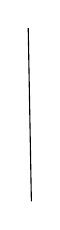
\begin{tikzpicture}[x=1cm,y=1cm]\draw (0.04,0)--(0,2.2);\end{tikzpicture}}}}
\uline{Corollaire} 7.2. Supposons que $k$ soit fini. Soit $S_d$ le schéma projectif défini par le vectoriel des formes de degré $d$ sur $P^r_k$. Alors pour tout ouvert non vide $U$ de $S_d$, et tout entier $a$, il existe un \inserted{\handwritten{point \deleted{fermé}}} $t\handwritten{\in}U\handwritten{(k')}$ \deleted{tel que}\inserted{\handwritten{(\unsure{avec|où} $k'$ une extension finie de $k$) tel que}}
% archive sheet number: 17
